\section{Cellular Security}

\subsection{1G: Analog}

\begin{itemize}
    \item Medium Access Control (MAC): Available bandwidth split using FDMA
    \item Connects Mobile Stations through Base Stations to the Mobile Telecommunications Switching Office.
    \item Handover protocol
    \item Essentially no security.
    \item Problem: Eavsdropping, Mobile cloning (billing fraud)
\end{itemize}

\subsection{2G: GSM}

\begin{itemize}
    \item Digital System
    \item Digital control channels: new features (SMS, Security mechanisms)
    \item GSM Global System for Mobile Communications
\end{itemize}

\begin{minipage}{\linewidth}
    \centering      
    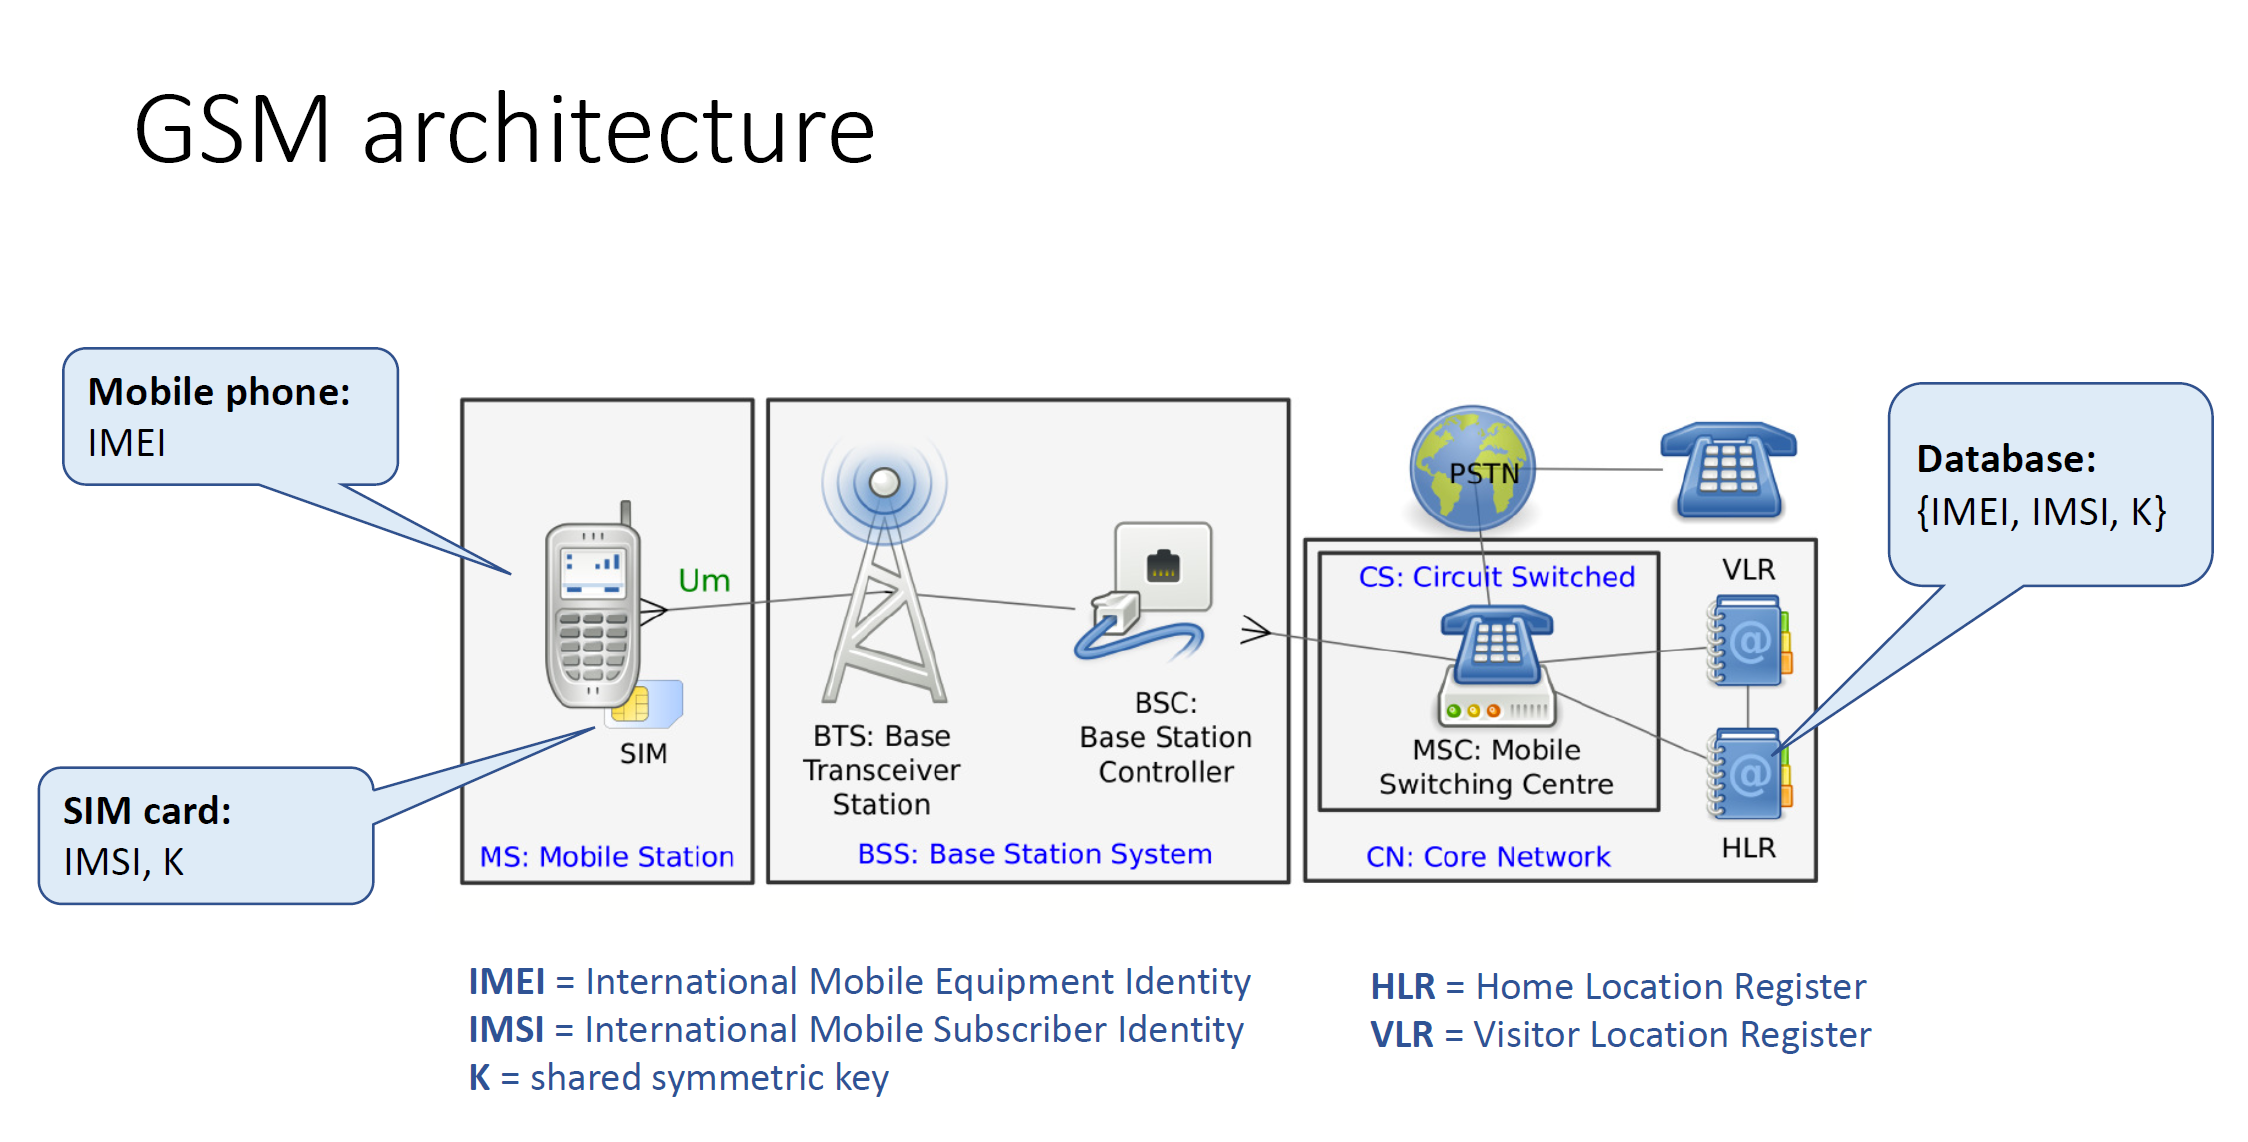
\includegraphics[width=\linewidth]{Figures/L10_gsm.PNG}
\end{minipage}

\paragraph{Security model}
\begin{itemize}
    \item All security based on symmetric shared keys
    \item GSM defines 3 Algorithms: A3 (auth), A8 (key deriv), A5 (encryption)
    \item Operators can choose A3 and A8 as they are on SIM
    \item No mutual authentication
    \item Encryption with fast Linear Shift Feedback Register (LSFR)
    
\end{itemize}

\paragraph{Problems}
\begin{itemize}
    \item Nohls attack, attack on A5 encryption with state tables (or rainbow tables): 
    Pre-compute chains, check if key matches. 
    Main enabler of this attack is 64 bit security.
    \item Attack on A8 (key derivation), recover Ki through side-channels, however operator can replace A8
    \item No integrity protection: GSM has no integrity protection, probably because of performance reasons. Adding MAC of 64 bits to each frame would lead to an overhead of 56\%. And also in voice channel modifications usually are not a problem.
    \item No mutual authentication: GSM does not authenticate Base station (b.c. Required equipment used to be very expensive for a BS). Calls encrypted limited damage. However, fake BS can identify and track user, and perform man in the middle attacks (we look at this later)
\end{itemize}

\subsection{SS7 Vulnerabilities}

\paragraph{SS7:} Signalling network 7 used in both GSM and 3G systems.
\begin{itemize}
    \item Protocol suite used to: route calls, coordinate roaming, deliver SMS
    \item Original trust model: walled garden, few participating operators and all trust each other, expensive equipment needed.
    \item GSM grew dramatically and cheap equipment appeared, original trust model no longer valid.
\end{itemize}

\paragraph{Location tracking:}
\begin{itemize}
    \item Get IMSI and address of current MSC (Mobile Switching Center)
    \item Request the cell id of the subscriber from the current MSC
    \item main enabler: Protocol Flaw in the GMLC
\end{itemize}

\paragraph{Intercepting Calls:}
\begin{enumerate}
    \item Attacker overwrites service control function's address with a fake one
    \item Attakcer can then redirect the call to a proxy relay which can then fully record the conversation. Man in the middle.
\end{enumerate} 

\subsection{3G: UMTS}
\begin{itemize}
    \item UMTS: Universal Mobile Telecommunications System
    \item W-CDMA wideband code-division multiple access, seperate spreading for each user
    \item New authentication and key agreement (AKA) protocol, mutual authentication, mutual replay protection.
    \item Integrity protection and encryption with KASUMI block cipher based on 8 rounds Feistel network, fast on hardware.
\end{itemize}

\begin{minipage}{\linewidth}
    \centering      
    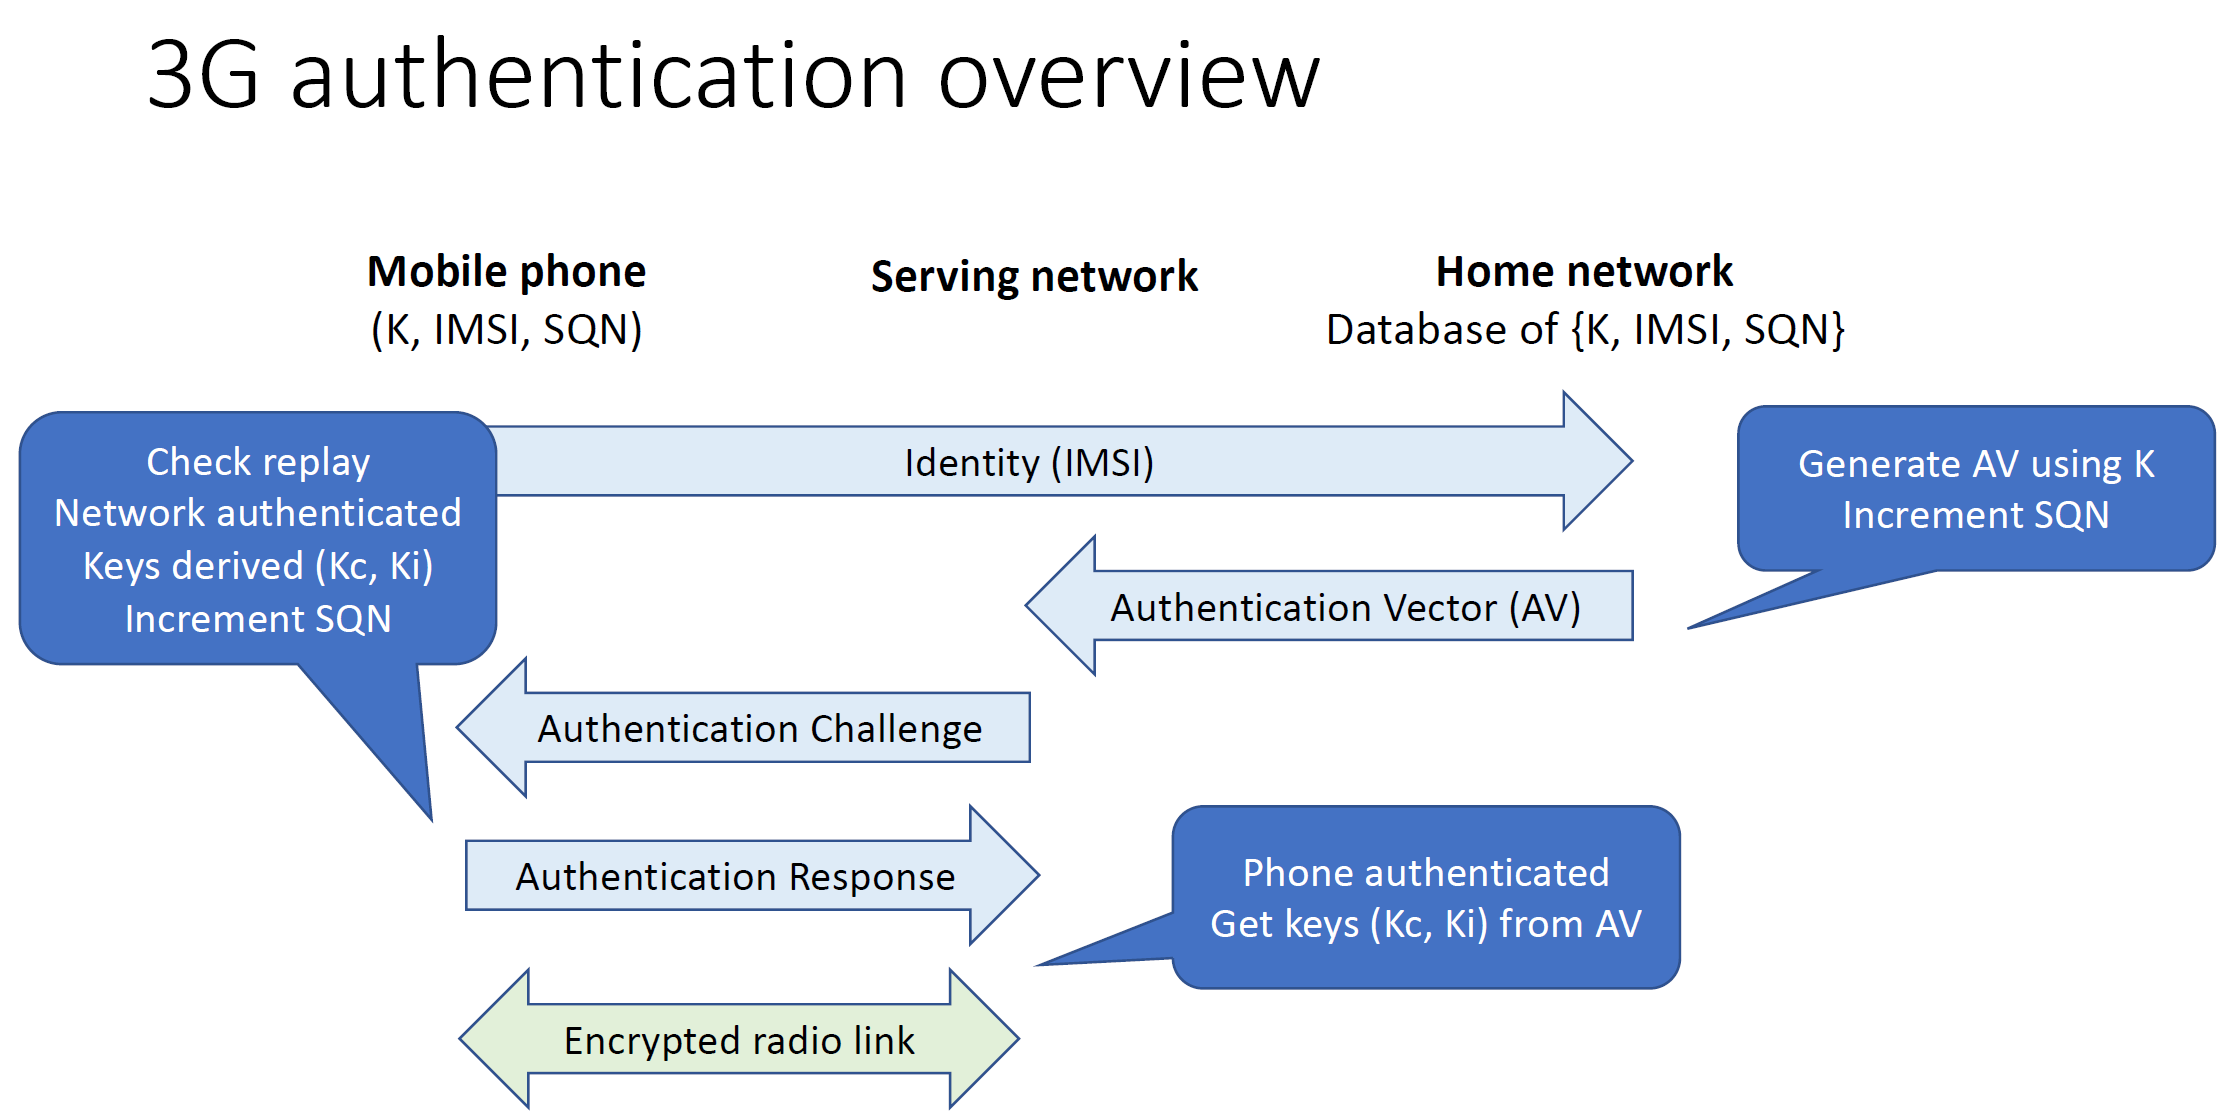
\includegraphics[width=\linewidth]{Figures/L10_3g_auth.PNG}
\end{minipage}

\paragraph{Denial of Service attack on 3g:} Use a cell phone jammer, cheap but illegal.
Also possible DoS attack on paging, as this takes place before authentication

\paragraph{Man in the middle (fake BS):}
\begin{itemize}
    \item 3G authentication (AKA) is mutual
    \item But we can use simple downgrade attack
\end{itemize}

\paragraph{Femtocells:} Operator provides small BS to customer to improve coverage in places like indoors. Problem is that they are considered trusted but provide much easier physical access for an attacker.

\paragraph{User tracking:}  In AKA mobile provides its identity (IMSI) before authentication, Operator assigns temporary identity (TMSI), user tracking possible to some extent. Fixes: dont send IMSI in plaintext or use pseudonyms at beginning of AKA.

\subsection{4G: LTE (Long Term Evolution)}

\paragraph{Overview:}
\begin{itemize}
    \item Orthogonal frequency division multiplex (OFDM)
    \item Multiple antenna techniques like MIMO
    \item Encryption usning AES-CTR, AES-CMAC
    \item Mutual authentication and SQN for replay detection
    \item The service area of operator divided into Tracking Areas (TAs)
    \item no integrity protection on user messages
    \item no confidentiality of paging
    \item no confidentiality on lower layers
\end{itemize}

\paragraph{Location tracking}
\begin{itemize}
    \item Enabler: GUTI reallocation depends on operator, availability was seen more important than privacy in this particular case.
    \item Setup fake BS
    \item Learn user presence in Tracking Area (TA)
    \item Learn precise location (fake BS sends unprotected RRC COnnection Reconfig
\end{itemize}

\paragraph{Man in the Middle}
\begin{enumerate}
    \item Learn user from encrypted traffic
    \item Modify encrypted traffic --> redirection. Deliver to false DNS server.
\end{enumerate}

\paragraph{Modify specific message bits attack:}
\begin{itemize}
    \item observe connection establishments in area
    \item learn many TMSIs
    \item page victim, isolate his TMSI
    \item record packet
    \item xor with whatever you want
    \item packet will be accepted because aes ctr does not authenticate
\end{itemize}

\begin{minipage}{\linewidth}
    \centering      
    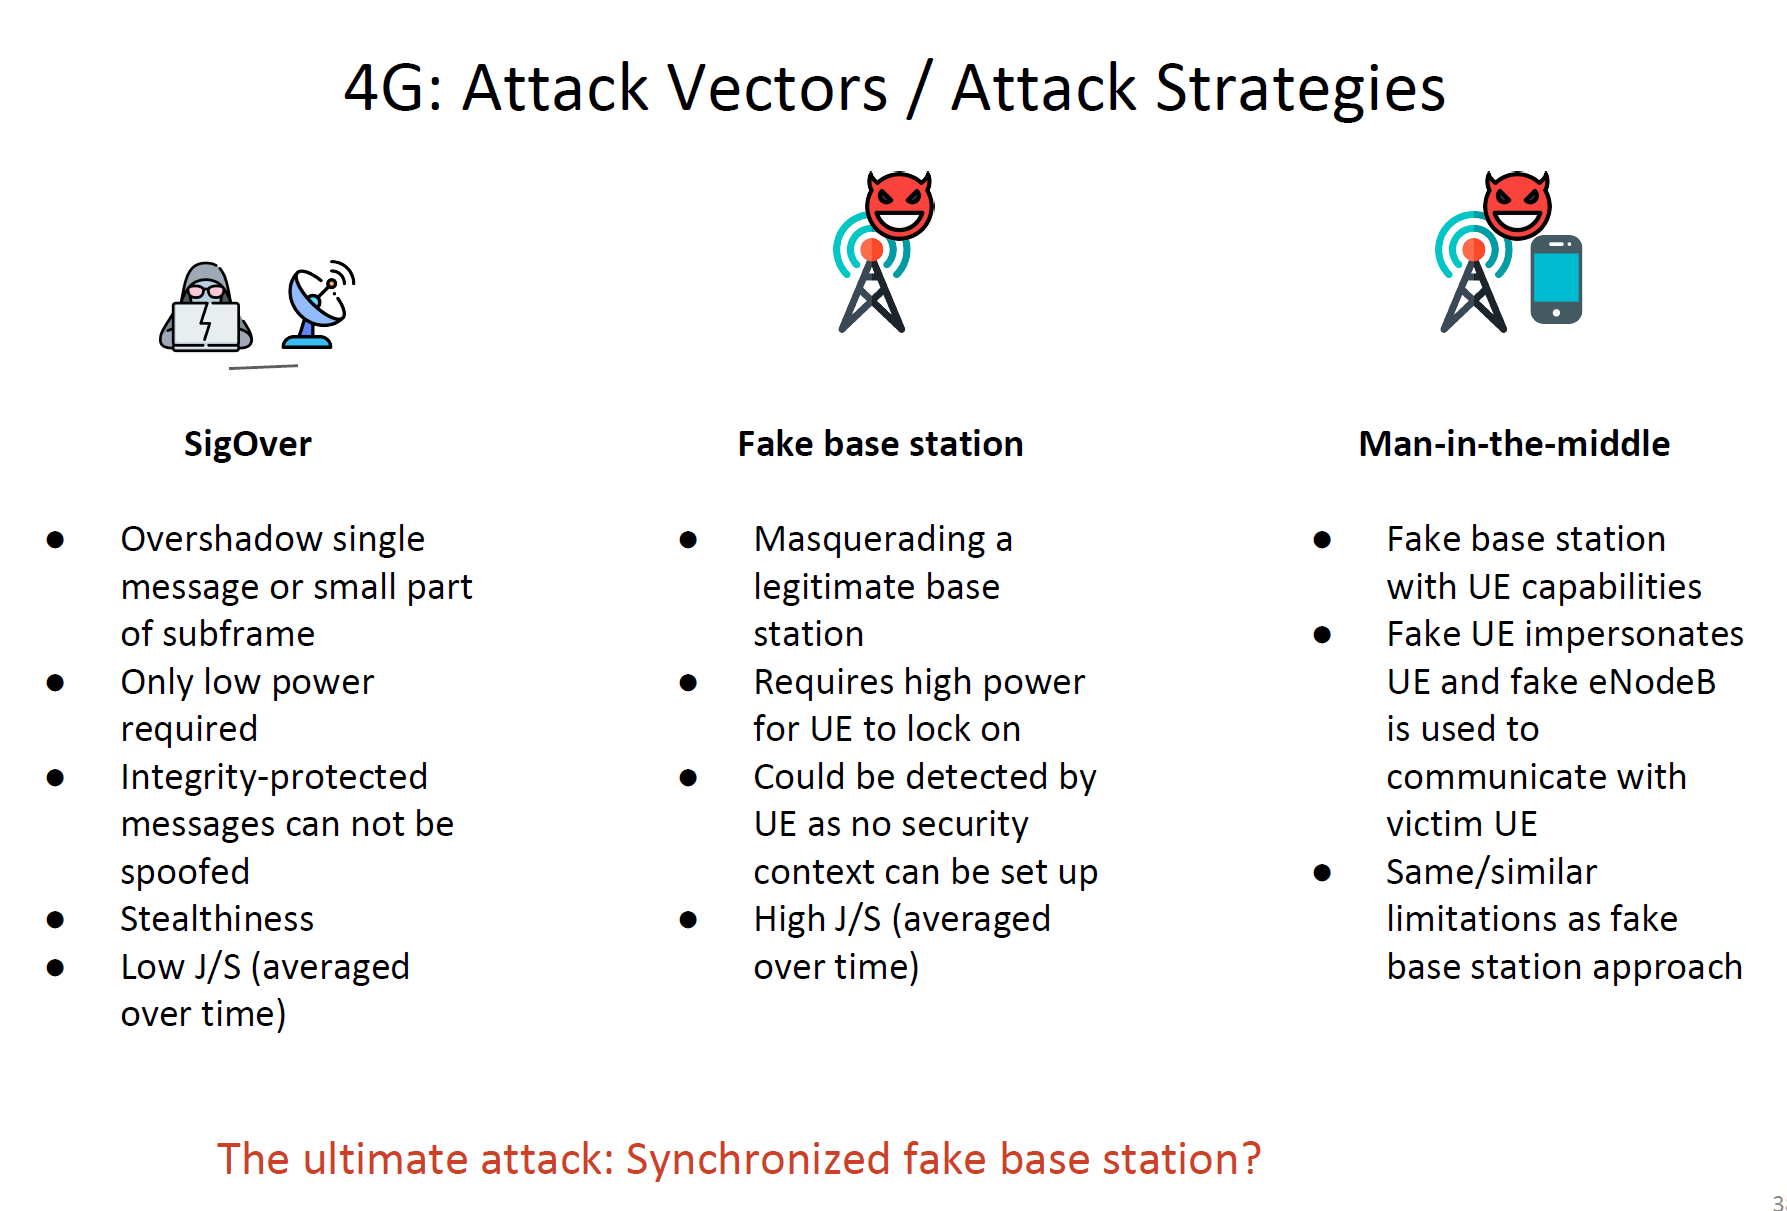
\includegraphics[width=\linewidth]{Figures/L10_lte_attacks.PNG}
\end{minipage}

